\section{Thuật toán Boyer-Moore}

Thuật toán tìm kiếm mẫu Boyer–Moore là một trong những thuật toán tìm kiếm chuỗi hiệu quả nhất và được xem như tiêu chuẩn đánh giá trong các bài toán đối sánh mẫu thực tế. Thuật toán này được phát triển bởi Robert Stephen Boyer và J Strother Moore vào năm 1977.

Thuật toán Boyer–Moore hoạt động bằng cách tiền xử lý xâu mẫu, sau đó quét văn bản từ phải sang trái, bắt đầu từ các ký tự ngoài cùng bên phải của mẫu. Thuật toán dựa trên nguyên tắc rằng nếu xảy ra sự không khớp, thì không cần phải kiểm tra các ký tự còn lại trong lần so khớp hiện tại. Cách tiếp cận theo hướng ngược này giúp giảm đáng kể độ phức tạp thời gian của thuật toán so với các phương pháp tìm kiếm chuỗi ngây thơ (naive).

Dưới đây là phần giải thích từng bước cách hoạt động của thuật toán Boyer–Moore:

\subsection{Tiền xử lý}

Thuật toán Boyer–Moore sử dụng hai heuristic (phương pháp kinh nghiệm) trong quá trình tiền xử lý mẫu:

\begin{itemize}
    \item Heuristic ký tự sai (Bad Character Heuristic)
    \item Heuristic hậu tố tốt (Good Suffix Heuristic)
\end{itemize}

\textbf{Heuristic ký tự sai (Bad Character Heuristic – xây dựng bảng ký tự sai)}

Heuristic này xác định khoảng dịch chuyển của mẫu khi xảy ra tình huống không khớp ký tự.

Thuật toán xây dựng một mảng (thường gọi là “bảng ký tự sai”) để lưu vị trí xuất hiện gần nhất (bên phải nhất) của mỗi ký tự trong mẫu. Nếu một ký tự không xuất hiện trong mẫu, giá trị của nó được gán bằng độ dài của mẫu.

Đối với mỗi ký tự trong mẫu, bảng được cập nhật theo vị trí xuất hiện cuối cùng của ký tự đó trong mẫu với công thức:

\[
BCT(ch) =
\begin{cases}
m & \text{if } ch \notin p \\
m - j - 1 & \text{otherwise}
\end{cases}
\]

Trong đó:
\begin{itemize}
    \item $m$ là độ dài của xâu mẫu $p$
    \item $j$ là vị trí xuất hiện cuối cùng của ký tự $ch$ trong xâu mẫu $p$
    \item $ch$ là ký tự đang xét trong bảng chữ cái
\end{itemize}

Ví dụ:

\begin{center}
    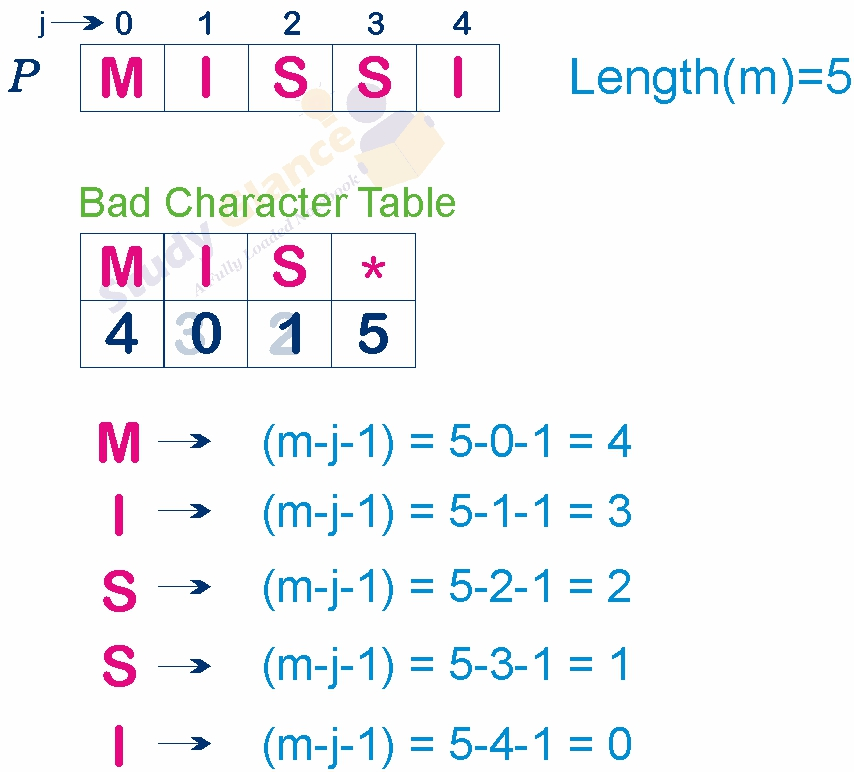
\includegraphics[width=12cm]{Images/Bad-Character-Table.jpg}
\end{center}

\subsection{Tìm kiếm}

Sau khi quá trình tiền xử lý hoàn tất, thuật toán bắt đầu bước tìm kiếm thực sự:

\begin{itemize}
    \item Căn chỉnh xâu mẫu với vị trí bắt đầu của văn bản.
    \item So sánh xâu mẫu với văn bản theo hướng từ phải sang trái.
    \item Nếu tất cả các ký tự trong xâu mẫu đều khớp với văn bản, thì một lần xuất hiện hợp lệ của mẫu đã được tìm thấy.
\end{itemize}

\subsection{Dịch chuyển mẫu (Shifting the Pattern)}
Khi xảy ra sự không khớp:

\begin{itemize}
    \item Nếu ký tự gây ra không khớp có xuất hiện trong mẫu, dịch chuyển mẫu sao cho ký tự đó trong văn bản được căn chỉnh với lần xuất hiện phải nhất của nó trong mẫu.
    \item Nếu ký tự gây ra không khớp không xuất hiện trong mẫu, dịch chuyển toàn bộ mẫu vượt qua ký tự đó trong văn bản.
\end{itemize}

\begin{center}
    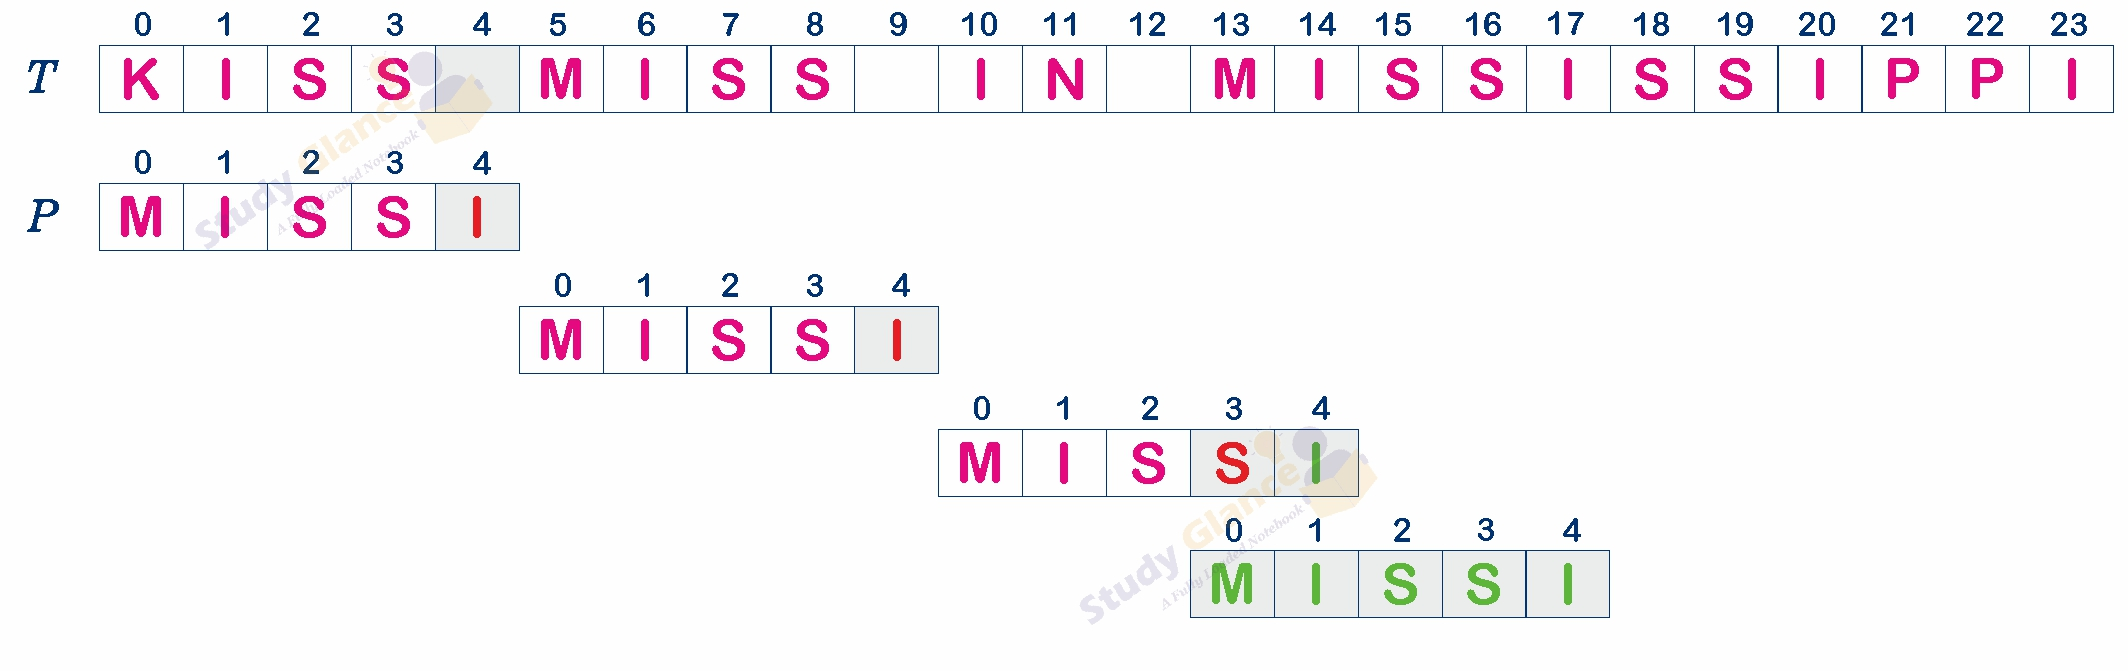
\includegraphics[width=12cm]{Images/Boyer-Moore-Algorithm-in-data-structures.jpg}
\end{center}

\subsection{Lặp lại quá trình so khớp}
Sau khi dịch chuyển mẫu theo các quy tắc đã nêu, thuật toán tiếp tục quá trình so sánh:

\begin{itemize}
    \item Tiếp tục so sánh xâu mẫu với văn bản theo hướng từ phải sang trái.
    \item Mỗi khi xảy ra sự không khớp, áp dụng các quy tắc dịch chuyển tương ứng.
    \item Quá trình này được lặp lại cho đến khi duyệt hết văn bản hoặc tìm được tất cả các vị trí xuất hiện của mẫu.
\end{itemize}

\subsection{Điều kiện kết thúc (Termination)}
Thuật toán kết thúc khi xảy ra một trong hai trường hợp sau:

\begin{itemize}
    \item Xâu mẫu đã được dịch chuyển vượt quá phần cuối của văn bản, nghĩa là không còn khả năng xuất hiện thêm kết quả khớp nào.
    \item Hoặc tất cả các lần xuất hiện của xâu mẫu trong văn bản đã được tìm thấy.
\end{itemize}

\subsection{Cài đặt thuật toán bằng C++}

\begin{verbatim}
#include <iostream>
#include <vector>
#include <string>
using namespace std;

#define NO_OF_CHARS 256

// Hàm xây dựng bảng Bad Character Heuristic
void buildBadCharTable(const string &pattern, vector<int> &badChar) {
    int m = pattern.size();

    // Khởi tạo tất cả giá trị = m
    for (int i = 0; i < NO_OF_CHARS; i++) {
        badChar[i] = m;
    }

    // Cập nhật vị trí xuất hiện cuối cùng
    for (int i = 0; i < m; i++) {
        badChar[(unsigned char)pattern[i]] = m - i - 1;
    }
}

// Hàm tìm kiếm Boyer-Moore (chỉ dùng Bad Character Heuristic)
vector<int> boyerMoore(string text, string pattern) {
    vector<int> result;

    int n = text.size();
    int m = pattern.size();

    vector<int> badChar(NO_OF_CHARS);

    buildBadCharTable(pattern, badChar);

    int shift = 0;

    while (shift <= n - m) {
        int j = m - 1;

        // So sánh từ phải sang trái
        while (j >= 0 && pattern[j] == text[shift + j]) {
            j--;
        }

        // Nếu khớp hoàn toàn
        if (j < 0) {
            result.push_back(shift);
            shift += (shift + m < n) ? m : 1;
        }
        else {
            // Dịch chuyển theo Bad Character Heuristic
            char bad = text[shift + j];
            shift += max(1, badChar[(unsigned char)bad] - (m - 1 - j));
        }
    }

    return result;
}

int main() {
    string text = "ababcabcabababd";
    string pattern = "ababd";

    vector<int> pos = boyerMoore(text, pattern);

    cout << "Vi tri xuat hien: ";
    for (int i : pos) {
        cout << i << " ";
    }

    return 0;
}
\end{verbatim}